
%% bare_conf.tex
%% V1.4b
%% 2015/08/26
%% by Michael Shell
%% See:
%% http://www.michaelshell.org/
%% for current contact information.
%%
%% This is a skeleton file demonstrating the use of IEEEtran.cls
%% (requires IEEEtran.cls version 1.8b or later) with an IEEE
%% conference paper.
%%
%% Support sites:
%% http://www.michaelshell.org/tex/ieeetran/
%% http://www.ctan.org/pkg/ieeetran
%% and
%% http://www.ieee.org/

%%*************************************************************************
%% Legal Notice:
%% This code is offered as-is without any warranty either expressed or
%% implied; without even the implied warranty of MERCHANTABILITY or
%% FITNESS FOR A PARTICULAR PURPOSE!
%% User assumes all risk.
%% In no event shall the IEEE or any contributor to this code be liable for
%% any damages or losses, including, but not limited to, incidental,
%% consequential, or any other damages, resulting from the use or misuse
%% of any information contained here.
%%
%% All comments are the opinions of their respective authors and are not
%% necessarily endorsed by the IEEE.
%%
%% This work is distributed under the LaTeX Project Public License (LPPL)
%% ( http://www.latex-project.org/ ) version 1.3, and may be freely used,
%% distributed and modified. A copy of the LPPL, version 1.3, is included
%% in the base LaTeX documentation of all distributions of LaTeX released
%% 2003/12/01 or later.
%% Retain all contribution notices and credits.
%% ** Modified files should be clearly indicated as such, including  **
%% ** renaming them and changing author support contact information. **
%%*************************************************************************


% *** Authors should verify (and, if needed, correct) their LaTeX system  ***
% *** with the testflow diagnostic prior to trusting their LaTeX platform ***
% *** with production work. The IEEE's font choices and paper sizes can   ***
% *** trigger bugs that do not appear when using other class files.       ***                          ***
% The testflow support page is at:
% http://www.michaelshell.org/tex/testflow/



\documentclass[conference]{IEEEtran}

\usepackage[pdftex]{graphicx}
\graphicspath{{../pdf/}{../jpeg/}}
\DeclareGraphicsExtensions{.pdf,.jpeg,.png}
% Some Computer Society conferences also require the compsoc mode option,
% but others use the standard conference format.
%
% If IEEEtran.cls has not been installed into the LaTeX system files,
% manually specify the path to it like:
% \documentclass[conference]{../sty/IEEEtran}





% Some very useful LaTeX packages include:
% (uncomment the ones you want to load)


% *** MISC UTILITY PACKAGES ***
%
%\usepackage{ifpdf}
% Heiko Oberdiek's ifpdf.sty is very useful if you need conditional
% compilation based on whether the output is pdf or dvi.
% usage:
% \ifpdf
%   % pdf code
% \else
%   % dvi code
% \fi
% The latest version of ifpdf.sty can be obtained from:
% http://www.ctan.org/pkg/ifpdf
% Also, note that IEEEtran.cls V1.7 and later provides a builtin
% \ifCLASSINFOpdf conditional that works the same way.
% When switching from latex to pdflatex and vice-versa, the compiler may
% have to be run twice to clear warning/error messages.






% *** CITATION PACKAGES ***
%
%\usepackage{cite}
% cite.sty was written by Donald Arseneau
% V1.6 and later of IEEEtran pre-defines the format of the cite.sty package
% \cite{} output to follow that of the IEEE. Loading the cite package will
% result in citation numbers being automatically sorted and properly
% "compressed/ranged". e.g., [1], [9], [2], [7], [5], [6] without using
% cite.sty will become [1], [2], [5]--[7], [9] using cite.sty. cite.sty's
% \cite will automatically add leading space, if needed. Use cite.sty's
% noadjust option (cite.sty V3.8 and later) if you want to turn this off
% such as if a citation ever needs to be enclosed in parenthesis.
% cite.sty is already installed on most LaTeX systems. Be sure and use
% version 5.0 (2009-03-20) and later if using hyperref.sty.
% The latest version can be obtained at:
% http://www.ctan.org/pkg/cite
% The documentation is contained in the cite.sty file itself.


\usepackage{url}



% *** GRAPHICS RELATED PACKAGES ***
%
\ifCLASSINFOpdf
  % \usepackage[pdftex]{graphicx}
  % declare the path(s) where your graphic files are
  % \graphicspath{{../pdf/}{../jpeg/}}
  % and their extensions so you won't have to specify these with
  % every instance of \includegraphics
  % \DeclareGraphicsExtensions{.pdf,.jpeg,.png}
\else
  % or other class option (dvipsone, dvipdf, if not using dvips). graphicx
  % will default to the driver specified in the system graphics.cfg if no
  % driver is specified.
  % \usepackage[dvips]{graphicx}
  % declare the path(s) where your graphic files are
  % \graphicspath{{../eps/}}
  % and their extensions so you won't have to specify these with
  % every instance of \includegraphics
  % \DeclareGraphicsExtensions{.eps}
\fi
% graphicx was written by David Carlisle and Sebastian Rahtz. It is
% required if you want graphics, photos, etc. graphicx.sty is already
% installed on most LaTeX systems. The latest version and documentation
% can be obtained at:
% http://www.ctan.org/pkg/graphicx
% Another good source of documentation is "Using Imported Graphics in
% LaTeX2e" by Keith Reckdahl which can be found at:
% http://www.ctan.org/pkg/epslatex
%
% latex, and pdflatex in dvi mode, support graphics in encapsulated
% postscript (.eps) format. pdflatex in pdf mode supports graphics
% in .pdf, .jpeg, .png and .mps (metapost) formats. Users should ensure
% that all non-photo figures use a vector format (.eps, .pdf, .mps) and
% not a bitmapped formats (.jpeg, .png). The IEEE frowns on bitmapped formats
% which can result in "jaggedy"/blurry rendering of lines and letters as
% well as large increases in file sizes.
%
% You can find documentation about the pdfTeX application at:
% http://www.tug.org/applications/pdftex





% *** MATH PACKAGES ***
%
%\usepackage{amsmath}
% A popular package from the American Mathematical Society that provides
% many useful and powerful commands for dealing with mathematics.
%
% Note that the amsmath package sets \interdisplaylinepenalty to 10000
% thus preventing page breaks from occurring within multiline equations. Use:
%\interdisplaylinepenalty=2500
% after loading amsmath to restore such page breaks as IEEEtran.cls normally
% does. amsmath.sty is already installed on most LaTeX systems. The latest
% version and documentation can be obtained at:
% http://www.ctan.org/pkg/amsmath





% *** SPECIALIZED LIST PACKAGES ***
%
%\usepackage{algorithmic}
% algorithmic.sty was written by Peter Williams and Rogerio Brito.
% This package provides an algorithmic environment fo describing algorithms.
% You can use the algorithmic environment in-text or within a figure
% environment to provide for a floating algorithm. Do NOT use the algorithm
% floating environment provided by algorithm.sty (by the same authors) or
% algorithm2e.sty (by Christophe Fiorio) as the IEEE does not use dedicated
% algorithm float types and packages that provide these will not provide
% correct IEEE style captions. The latest version and documentation of
% algorithmic.sty can be obtained at:
% http://www.ctan.org/pkg/algorithms
% Also of interest may be the (relatively newer and more customizable)
% algorithmicx.sty package by Szasz Janos:
% http://www.ctan.org/pkg/algorithmicx




% *** ALIGNMENT PACKAGES ***
%
%\usepackage{array}
% Frank Mittelbach's and David Carlisle's array.sty patches and improves
% the standard LaTeX2e array and tabular environments to provide better
% appearance and additional user controls. As the default LaTeX2e table
% generation code is lacking to the point of almost being broken with
% respect to the quality of the end results, all users are strongly
% advised to use an enhanced (at the very least that provided by array.sty)
% set of table tools. array.sty is already installed on most systems. The
% latest version and documentation can be obtained at:
% http://www.ctan.org/pkg/array


% IEEEtran contains the IEEEeqnarray family of commands that can be used to
% generate multiline equations as well as matrices, tables, etc., of high
% quality.




% *** SUBFIGURE PACKAGES ***
%\ifCLASSOPTIONcompsoc
%  \usepackage[caption=false,font=normalsize,labelfont=sf,textfont=sf]{subfig}
%\else
%  \usepackage[caption=false,font=footnotesize]{subfig}
%\fi
% subfig.sty, written by Steven Douglas Cochran, is the modern replacement
% for subfigure.sty, the latter of which is no longer maintained and is
% incompatible with some LaTeX packages including fixltx2e. However,
% subfig.sty requires and automatically loads Axel Sommerfeldt's caption.sty
% which will override IEEEtran.cls' handling of captions and this will result
% in non-IEEE style figure/table captions. To prevent this problem, be sure
% and invoke subfig.sty's "caption=false" package option (available since
% subfig.sty version 1.3, 2005/06/28) as this is will preserve IEEEtran.cls
% handling of captions.
% Note that the Computer Society format requires a larger sans serif font
% than the serif footnote size font used in traditional IEEE formatting
% and thus the need to invoke different subfig.sty package options depending
% on whether compsoc mode has been enabled.
%
% The latest version and documentation of subfig.sty can be obtained at:
% http://www.ctan.org/pkg/subfig




% *** FLOAT PACKAGES ***
%
%\usepackage{fixltx2e}
% fixltx2e, the successor to the earlier fix2col.sty, was written by
% Frank Mittelbach and David Carlisle. This package corrects a few problems
% in the LaTeX2e kernel, the most notable of which is that in current
% LaTeX2e releases, the ordering of single and double column floats is not
% guaranteed to be preserved. Thus, an unpatched LaTeX2e can allow a
% single column figure to be placed prior to an earlier double column
% figure.
% Be aware that LaTeX2e kernels dated 2015 and later have fixltx2e.sty's
% corrections already built into the system in which case a warning will
% be issued if an attempt is made to load fixltx2e.sty as it is no longer
% needed.
% The latest version and documentation can be found at:
% http://www.ctan.org/pkg/fixltx2e


%\usepackage{stfloats}
% stfloats.sty was written by Sigitas Tolusis. This package gives LaTeX2e
% the ability to do double column floats at the bottom of the page as well
% as the top. (e.g., "\begin{figure*}[!b]" is not normally possible in
% LaTeX2e). It also provides a command:
%\fnbelowfloat
% to enable the placement of footnotes below bottom floats (the standard
% LaTeX2e kernel puts them above bottom floats). This is an invasive package
% which rewrites many portions of the LaTeX2e float routines. It may not work
% with other packages that modify the LaTeX2e float routines. The latest
% version and documentation can be obtained at:
% http://www.ctan.org/pkg/stfloats
% Do not use the stfloats baselinefloat ability as the IEEE does not allow
% \baselineskip to stretch. Authors submitting work to the IEEE should note
% that the IEEE rarely uses double column equations and that authors should try
% to avoid such use. Do not be tempted to use the cuted.sty or midfloat.sty
% packages (also by Sigitas Tolusis) as the IEEE does not format its papers in
% such ways.
% Do not attempt to use stfloats with fixltx2e as they are incompatible.
% Instead, use Morten Hogholm'a dblfloatfix which combines the features
% of both fixltx2e and stfloats:
%
% \usepackage{dblfloatfix}
% The latest version can be found at:
% http://www.ctan.org/pkg/dblfloatfix




% *** PDF, URL AND HYPERLINK PACKAGES ***
%
%\usepackage{url}
% url.sty was written by Donald Arseneau. It provides better support for
% handling and breaking URLs. url.sty is already installed on most LaTeX
% systems. The latest version and documentation can be obtained at:
% http://www.ctan.org/pkg/url
% Basically, \url{my_url_here}.




% *** Do not adjust lengths that control margins, column widths, etc. ***
% *** Do not use packages that alter fonts (such as pslatex).         ***
% There should be no need to do such things with IEEEtran.cls V1.6 and later.
% (Unless specifically asked to do so by the journal or conference you plan
% to submit to, of course. )


% correct bad hyphenation here
\hyphenation{op-tical net-works semi-conduc-tor}


\begin{document}
%
% paper title
% Titles are generally capitalized except for words such as a, an, and, as,
% at, but, by, for, in, nor, of, on, or, the, to and up, which are usually
% not capitalized unless they are the first or last word of the title.
% Linebreaks \\ can be used within to get better formatting as desired.
% Do not put math or special symbols in the title.
\title{Prototyping Resilient Processing Cores in Workcraft}

% author names and affiliations
% use a multiple column layout for up to three different
% affiliations
\author{\IEEEauthorblockN{Georgy Lukyanov}
\IEEEauthorblockA{
Southern Federal University\\
Rostov-on-Don, Russia\\}
\and
\IEEEauthorblockN{Alessandro de Gennaro\\Paulius Stankaitis\\Andrey Mokhov}
\IEEEauthorblockA{\\Newcastle University\\
Newcastle, UK}
\and
\IEEEauthorblockN{\\Maxim Rykunov\\}
\IEEEauthorblockA{\\\\IMEC\\
Leuven, Belgium}}

% conference papers do not typically use \thanks and this command
% is locked out in conference mode. If really needed, such as for
% the acknowledgment of grants, issue a \IEEEoverridecommandlockouts
% after \documentclass

% for over three affiliations, or if they all won't fit within the width
% of the page, use this alternative format:
%
%\author{\IEEEauthorblockN{Michael Shell\IEEEauthorrefmark{1},
%Homer Simpson\IEEEauthorrefmark{2},
%James Kirk\IEEEauthorrefmark{3},
%Montgomery Scott\IEEEauthorrefmark{3} and
%Eldon Tyrell\IEEEauthorrefmark{4}}
%\IEEEauthorblockA{\IEEEauthorrefmark{1}School of Electrical and Computer Engineering\\
%Georgia Institute of Technology,
%Atlanta, Georgia 30332--0250\\ Email: see http://www.michaelshell.org/contact.html}
%\IEEEauthorblockA{\IEEEauthorrefmark{2}Twentieth Century Fox, Springfield, USA\\
%Email: homer@thesimpsons.com}
%\IEEEauthorblockA{\IEEEauthorrefmark{3}Starfleet Academy, San Francisco, California 96678-2391\\
%Telephone: (800) 555--1212, Fax: (888) 555--1212}
%\IEEEauthorblockA{\IEEEauthorrefmark{4}Tyrell Inc., 123 Replicant Street, Los Angeles, California 90210--4321}}


% use for special paper notices
%\IEEEspecialpapernotice{(Invited Paper)}


% make the title area
\maketitle

% As a general rule, do not put math, special symbols or citations
% in the abstract
\begin{abstract}
We present a methodology for the design and fast prototyping of
processing cores with resilient microarchitecture. The resilience is
achieved by equipping the core with a family of datapath components
optimised for different operating modes and a flexible control
structure that allows to change an instruction implementation in
runtime depending on the environmental conditions and application
requirements. We use asynchronous design techniques to achieve
\emph{short-term resilience}, i.e. survival in extreme environmental
conditions, such as near-threshold and/or unstable voltage supply.
\emph{Long-term resilience} is achieved by providing mechanisms for
runtime reconfiguration of the processor microarchitecture, which
is essential for safety-critical applications, such as biomedical
implants that cannot be taken offline for maintenance. By using
formal methods one can guarantee the correctness and uninterrupted
service during such runtime reconfigurations.

The presented methodology is supported by open-source EDA tool
Workcraft, and has been validated in silicon by successfully
fabricating two chips: Intel 8051 processing core and a
reconfigurable dataflow pipeline for ordinal pattern analysis.
To facilitate fast prototyping of resilient processing cores, we
propose a domain-specific language for formal specification,
compiler-checked documentation, and software-level simulation of
processor prototypes.
\end{abstract}

% no keywords


% For peer review papers, you can put extra information on the cover
% page as needed:
% \ifCLASSOPTIONpeerreview
% \begin{center} \bfseries EDICS Category: 3-BBND \end{center}
% \fi
%
% For peerreview papers, this IEEEtran command inserts a page break and
% creates the second title. It will be ignored for other modes.
\IEEEpeerreviewmaketitle

\newpage	
\section{Formal methods for runtime reconfigurability}


%Systems reconfigurability is paramount for a number of safety critical systems classes.  
%In general complex dependable systems must be self-adaptive to continually 
%changing environment and ideally reconfigure dynamically without any 
%human intervention.   

%use mathematical approach.%\cite{calinescu2010formal}

Formal methods - a mathematical model driven method provides a systematic approach
for developing complex systems in a design reusable and correct-by-construction
manner. The suitability of these techniques for a specification and verification of
dynamically reconfigurable systems has been studied for some time now. A survey by 
Calinescu and Kikuchi \cite{calinescu2010formal} overviews possible approaches in 
using formal methods for adaptive systems at runtime. In an empirical comparison
study by Bhattacharyya et al. \cite{DBLP:journals/corr/BhattacharyyaMP16}  different 
formalisms for modelling suitability of reconfigurable systems were explored. The authors of the paper 
\cite{Weyns:2012:SFM:2347583.2347592} review a decade of research on formal 
methods for adaptive systems. Even though the formal verification is traditionally 
an off-line procedure some progress have been achieved in integrating techniques like 
model checking at runtime. The model checking approach involves specifying system behaviour
formally or else using a model finding approach \cite{kikuchi2010configuration} 
and exhaustively checking that systems properties hold at every system change. 
The counter-examples can be used to resolve the policy conflicts as discussed by
Calinescu and Kikuchi in their paper. The other methods include using a mathematical logic and theorem prover  
to verify dynamic reconfiguration of cores at a runtime \cite{singh1999formal}. The proposed schema
automatically generates the new specification of the system in a propositional logic and calls
the theorem prover at the runtime to check the correctness. A lot of safety critical systems
system has to preserve requirements for resources in case of system failures and in many instances this requires 
reasoning in discrete-continuous domain which is best captured with hybrid models.
A generic substitution model has been introduced by Babin et al. to reason about reconfigurable
systems where system state has to be preserved \cite{Babin2016}. The biggest challenge in
integrating formal verification at runtime is the tool scalability as particularly for
model checking state-space explosion remains a big challenge.

In the our work we introduced a formal model for analysing dynamically reconfigurable control
systems \cite{mokhov2008conditional} and presented how verification conditions for our
model can be expressed as SAT-problems \cite{mokhov2008verification}. 

 %suitable models for analysing
 %discrete-continuous systems are hybrid models. A lot of work has been done to allow
 %modelling such a complex systems and one of the generic models for reconfigurable
 %systems is presented by Babin et al. with a case study for maintaining safe energy
 %level \cite{Babin2016}. The future work direction could involve integrating a similiar
 %approach within our graph-based model.
%Runtime systems adaptation is currently one the biggest challenges in formal
%methods community. 
%A number of formal models exists for specification of process-based systems for
%instance Petri nets \cite{peterson1981petri} or Finite State Machines
%\cite{nowick1993automatic} or else hardware description languages such as Verilog or
% VHDL. The majority of industrial projects used formal techniques exactly for the
%specification and modelling as has been shown by Woodcock et al.
%\cite{woodcock2009formal}. The description of application (even formal) is not
%ufficient to evidently demonstrate reliability of the system. The development
%process must be accompanied with a form formal verification and mainly there exists
%two formal verification techniques - theorem proving and model checking. The
%principal of the model checking is to construct a finite-state model and by
%exploring state-space exhaustively check whether the model meets requirements. The
%alternative technique for automated verification is automated theorem proving which
%does not rely on exploring the state-space. The benefits of automated theorem
%proving in hardware design validation are increasingly recognised by the embedded
%system industry \cite{clarke1996formal} and several companies have already
%integrated tools like ACL2 or Isabelle into application development process
%\cite{kaufmann2004some}. 



%Our graph-based
%approach combines advantages of PNs and FSMs are is able of capturing concurrency
%and choice in a compact and efficient way. 

%A lot of changes in the system happens due
%to the environment (plant) changes and the most


\newpage
\section{Using Domain-Specific Languages to improve the 
productivity of REES designers}

Domain-Specific Languages (DSLs) are designed to have maximal expression for
tasks of particular field, such as VHDL for hardware description or \LaTeX~for 
typesetting. However, implementing a language from scratch may be tedious, 
time-consuming and error-prone. Therefore, especially for prototyping purposes, 
DSLs could be embedded into existing general-purpose programming language.
Modern typed functional programming languages such as Haskell offer a wide range
of facilities for construction of embedded domain-specific languages (EDSLs) 
that could benefit from features of lightweight verification provided by rich 
type system and highly-tailored syntax achieved using various functional 
programming idioms.

In order to produce robust hardware, its vital to have qualitative formal
specification methods, simulation facilities, and verifications techniques.
EDSLs may come in handy on every stage of hardware design: specification
languages help to describe system functions in a declarative way, software
simulation environment gives a possibility to evaluate system capabilities
without building an expensive prototype, and advanced types of hosting language
encoding initial system specification provide verified-by-construction result. 

Workcraft framework provide three DSLs: 

\begin{itemize}
\item Signal Transition Graphs (STGs) --- a low-level (signal-level) DSL for 
specifying resilient asynchronous controllers.
\item Conditional Partial Order Graphs (CPOGs) --- an intermediate-level 
(microarchitecture-level) DSL for specifying processor instructions as 
collections of partial orders.
\item Dataflow Structures (DFSs) --- an intermediate-level (dataflow graphs) DSL 
for specifying reconfigurable dataflow graphs.
\end{itemize}

Workcraft is able to translate models described with support of these DSLs into 
Verilog --- a standard low-level industrial design language for hardware 
description.  

In our work, we concentrate on bridging Event-B --- a high-level DSL
for formal specification of system requirements and system reconfiguration, 
supported by Rodin toolset, and DSLs provided by Workcraft. As a 
prototype of a bridging language, we develop Farfalle --- 
an intermediate-level DSL embedded into Haskell that 
is focused on description of processor microarchitectures.
Haskell provide a very expressive tools for description of data and 
computations. A concept of \texttt{Monad} gives a powerful abstraction for 
building customized type-safe EDSLs, and syntactical support for monadic 
\texttt{do}-notation makes this embedding perfectly smooth. Therefore, Farfalle
has means to reduce errors in resilient systems design and give engineers a fast 
and safe prototyping tool.      


\section{Tool support}

Formalising the design specifications is a good approach to the development of a resilient
system. Specifications, represented via DSL, can indeed be verified and
simulated, targeting an error-free system. Workcraft~\cite{workcraft_web} provides the support for different
models, this can help the design for resiliency. Conditional partial order graphs (CPOG)~\cite{CPOG}
(available in the Workcraft framework), for instance, can support the development of
processor instruction sets. In Figure \ref{fig:screenshot}, all the steps from the
specification of each instruction, to the synthesis of the final microcontroller are
depicted. Instructions can be specified in the form of algebraic equations at first, then the
graphs can be imported, encoded and synthesised in the form of a microcontroller. The latter
can be mapped with the usage of a technology library and eventually simulated: internal and
external signals can be visualised via digital waveforms, where dependencies among signals
are shown. we are developing a DSL for bridging the gap between formal methods toolsets such
Rodin and hardware synthesis toolsets such as Workcraft. Having a scalable, yet
reusable language would be beneficial for resiliency. The instruction correctness, indeed,
could be simulated and formally verified, the partial order should be derived from the
specifications.

\begin{figure*}[ht!]
\begin{center}
	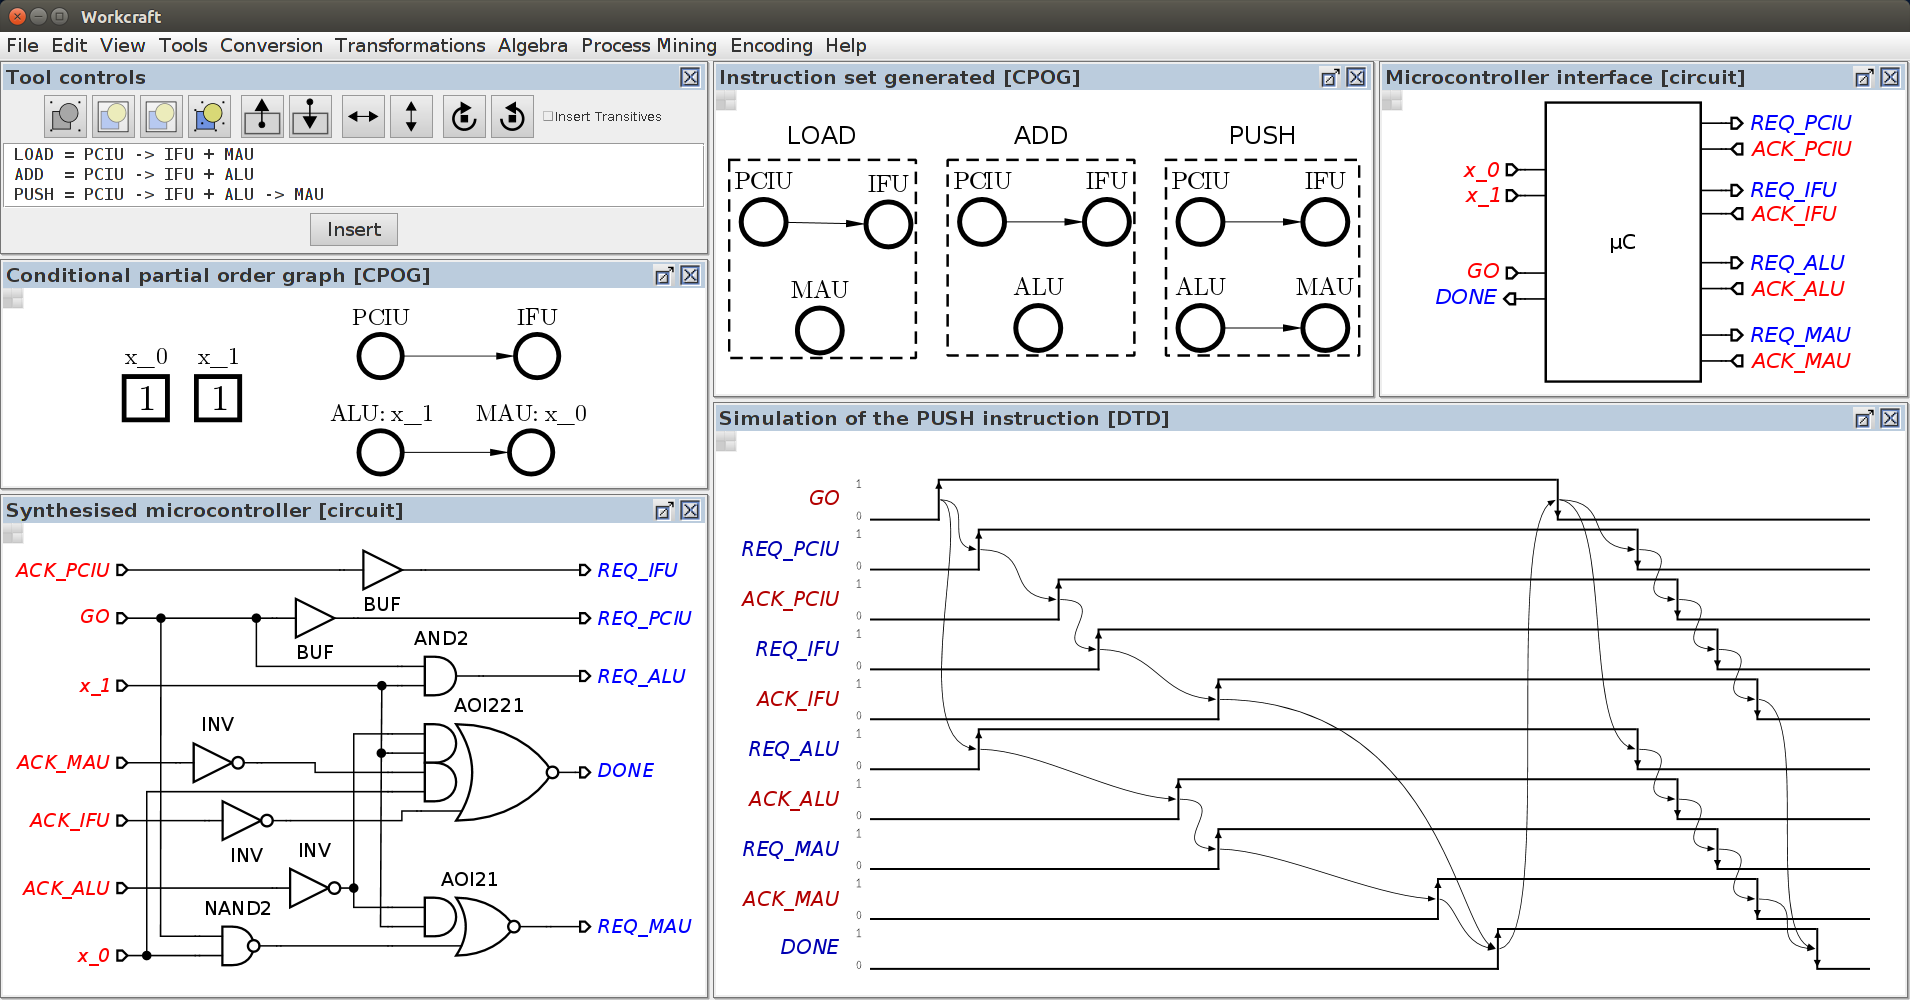
\includegraphics[width=\linewidth]{FIG/screen.png}
	\caption{From the specification of the partial orders, to the synthesis and simulation
	of the microcontroller. Screenshot from Workcraft.}
	\label{fig:screenshot}
\end{center}
\end{figure*}

The CPOG and Dataflow Structures (DFS)~\cite{DFS} were used together to design an asynchronous
reconfigurable pipeline for the computation of the ordinal pattern encoding~\cite{OPE}. CPOG was used
for the design of the control unit, which is used for the reconfigurability of the pipeline
(3-18 stages). DFS supported the design of the datapath asynchronous components instead. Each
module has indeed been modelled and simulated in Workcraft at first, and then translated into
hardware description (Verilog). The DFS model matches the HDL description, the asynchronous
4-phase dual rail protocol is implemented. Figure \ref{fig:voltage-resiliency} shows the
resiliency of the chip to the voltage variation. Workcraft, and the tools that the framework
comes with, have been also validated with the design of an asynchronous processor (Intel
8051~\cite{rec-proc}), the flow can still be improved by adopting DSL for formalising system
specifications.

\begin{figure}[ht!]
\begin{center}
	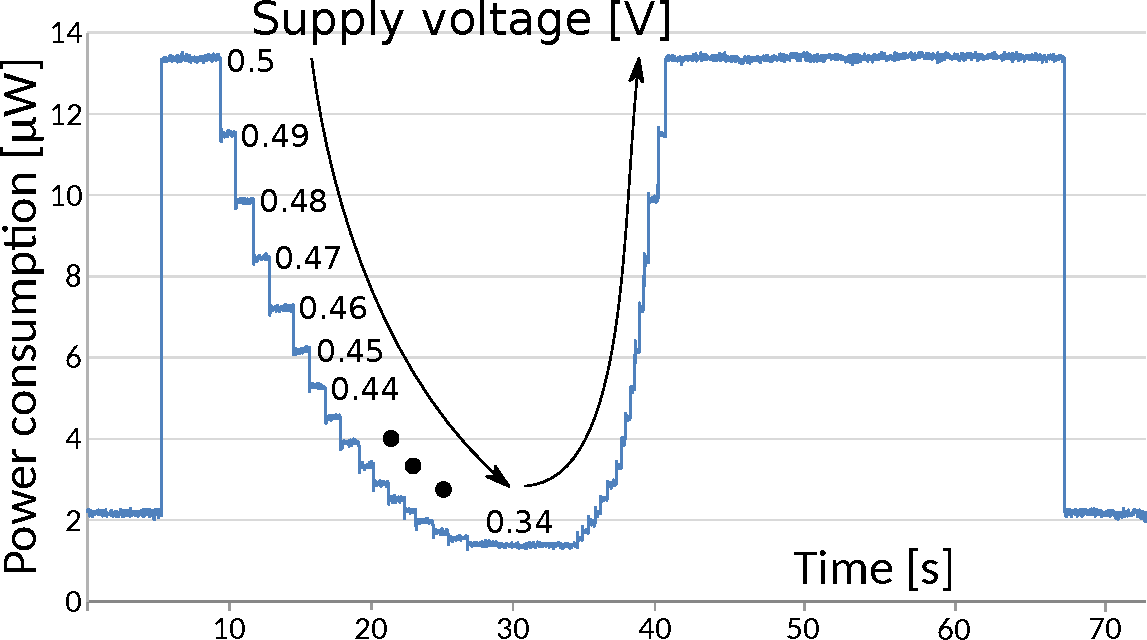
\includegraphics[width=\linewidth]{FIG/ope-chip.pdf}
	\caption{Voltage resiliency of the asynchronous reconfigurable pipeline, implemented in
	an ASIC with the 90nm TSMC technology.}
	\label{fig:voltage-resiliency}
\end{center}
\end{figure}

% An example of a floating figure using the graphicx package.
% Note that \label must occur AFTER (or within) \caption.
% For figures, \caption should occur after the \includegraphics.
% Note that IEEEtran v1.7 and later has special internal code that
% is designed to preserve the operation of \label within \caption
% even when the captionsoff option is in effect. However, because
% of issues like this, it may be the safest practice to put all your
% \label just after \caption rather than within \caption{}.
%
% Reminder: the "draftcls" or "draftclsnofoot", not "draft", class
% option should be used if it is desired that the figures are to be
% displayed while in draft mode.
%
%\begin{figure}[!t]
%\centering
%\includegraphics[width=2.5in]{myfigure}
% where an .eps filename suffix will be assumed under latex,
% and a .pdf suffix will be assumed for pdflatex; or what has been declared
% via \DeclareGraphicsExtensions.
%\caption{Simulation results for the network.}
%\label{fig_sim}
%\end{figure}

% Note that the IEEE typically puts floats only at the top, even when this
% results in a large percentage of a column being occupied by floats.


% An example of a double column floating figure using two subfigures.
% (The subfig.sty package must be loaded for this to work.)
% The subfigure \label commands are set within each subfloat command,
% and the \label for the overall figure must come after \caption.
% \hfil is used as a separator to get equal spacing.
% Watch out that the combined width of all the subfigures on a
% line do not exceed the text width or a line break will occur.
%
%\begin{figure*}[!t]
%\centering
%\subfloat[Case I]{\includegraphics[width=2.5in]{box}%
%\label{fig_first_case}}
%\hfil
%\subfloat[Case II]{\includegraphics[width=2.5in]{box}%
%\label{fig_second_case}}
%\caption{Simulation results for the network.}
%\label{fig_sim}
%\end{figure*}
%
% Note that often IEEE papers with subfigures do not employ subfigure
% captions (using the optional argument to \subfloat[]), but instead will
% reference/describe all of them (a), (b), etc., within the main caption.
% Be aware that for subfig.sty to generate the (a), (b), etc., subfigure
% labels, the optional argument to \subfloat must be present. If a
% subcaption is not desired, just leave its contents blank,
% e.g., \subfloat[].


% An example of a floating table. Note that, for IEEE style tables, the
% \caption command should come BEFORE the table and, given that table
% captions serve much like titles, are usually capitalized except for words
% such as a, an, and, as, at, but, by, for, in, nor, of, on, or, the, to
% and up, which are usually not capitalized unless they are the first or
% last word of the caption. Table text will default to \footnotesize as
% the IEEE normally uses this smaller font for tables.
% The \label must come after \caption as always.
%
%\begin{table}[!t]
%% increase table row spacing, adjust to taste
%\renewcommand{\arraystretch}{1.3}
% if using array.sty, it might be a good idea to tweak the value of
% \extrarowheight as needed to properly center the text within the cells
%\caption{An Example of a Table}
%\label{table_example}
%\centering
%% Some packages, such as MDW tools, offer better commands for making tables
%% than the plain LaTeX2e tabular which is used here.
%\begin{tabular}{|c||c|}
%\hline
%One & Two\\
%\hline
%Three & Four\\
%\hline
%\end{tabular}
%\end{table}


% Note that the IEEE does not put floats in the very first column
% - or typically anywhere on the first page for that matter. Also,
% in-text middle ("here") positioning is typically not used, but it
% is allowed and encouraged for Computer Society conferences (but
% not Computer Society journals). Most IEEE journals/conferences use
% top floats exclusively.
% Note that, LaTeX2e, unlike IEEE journals/conferences, places
% footnotes above bottom floats. This can be corrected via the
% \fnbelowfloat command of the stfloats package.


% trigger a \newpage just before the given reference
% number - used to balance the columns on the last page
% adjust value as needed - may need to be readjusted if
% the document is modified later
%\IEEEtriggeratref{8}
% The "triggered" command can be changed if desired:
%\IEEEtriggercmd{\enlargethispage{-5in}}

% references section

% can use a bibliography generated by BibTeX as a .bbl file
% BibTeX documentation can be easily obtained at:
% http://mirror.ctan.org/biblio/bibtex/contrib/doc/
% The IEEEtran BibTeX style support page is at:
% http://www.michaelshell.org/tex/ieeetran/bibtex/
%\bibliographystyle{IEEEtran}
% argument is your BibTeX string definitions and bibliography database(s)
%\bibliography{IEEEabrv,../bib/paper}
%
% <OR> manually copy in the resultant .bbl file
% set second argument of \begin to the number of references
% (used to reserve space for the reference number labels box)

\begin{thebibliography}{10}

\bibitem{CPOG}
	A. Mokhov, A. Yakovlev. \emph{``Conditional partial order graphs: Model, 
	synthesis, and application''}. IEEE Transactions on Computers, Volume 59,
	Pages 1480-1493, November 2010.
	
\bibitem{workcraft_web}
	\textsc{Workcraft} homepage. \url{http://www.workcraft.org/}.	
	
\bibitem{DFS}
	D. Sokolov, I. Poliakov, A. Yakovlev. \emph{``Analysis of static data flow structures''}.
	Fundamenta Informaticae, volume 88,issue 4, pages 581 - 610. Publisher IOS Press. 2008.

\bibitem{OPE}
	C. Guo, W. Luk, S. Weston:
	\emph{``Pipelined reconfigurable accelerator for ordinal pattern encoding''}.
	Proc. Application-specific Systems, Architectures and Processors~(ASAP),
	pp.~194--201, 2014.
	
\bibitem{rec-proc}
	A. Mokhov, M. Rykunov, D. Sokolov, A. Yakovlev.
	\emph{``Design of Processors with Reconfigurable Microarchitecture''}.
	J. Low Power Electronics Application 2014, Volume 4(1). Pages 26-43.

\bibitem{calinescu2010formal}
R. Calinescu, S. Kikuchi. \emph{``Formal methods@ runtime''}. In Proceedings of the Monterey
Workshop, Pages 122–135, Springer, 2010.

\bibitem{DBLP:journals/corr/BhattacharyyaMP16}
A. Bhattacharyya, A. Mokhov, K. Pierce. \emph{``An Empirical Comparison of Formalisms for Modelling and Analysis of
	Dynamic Reconfiguration of Dependable Systems''}. CoRR, Volume abs/1609.08531, 2016.

\bibitem{Weyns:2012:SFM:2347583.2347592}
D. Weyns, M. U. Iftikhar, D. G. de la Iglesia, T. Ahmad. \emph{``A
survey of formal methods in self-adaptive systems''}. In Proceedings of the International C* Conference on 
Computer Science and Software Engineering, C3S2E ’12, (New York, NY, USA), Pages 67–79, ACM, 2012.

\bibitem{kikuchi2010configuration}
S. Kikuchi, S. Tsuchiya. \emph{``Configuration procedure synthesis for complex systems using model finder''}. 
In Proceedings of the 15th IEEE International Conference on Engineering of Complex Computer 
Systems (ICECCS), Pages 95–104, IEEE, 2010.

\bibitem{singh1999formal}
S. Singh, C. J. Lillieroth. \emph{``Formal verification of reconfigurable core''}. 
Seventh Annual IEEE Symposium on Field-Programmable Custom Computing Machines, 1999. FCCM’99. 
Proceedings. , Pages 25–32, IEEE, 1999.

\bibitem{Babin2016}
G. Babin, Y. A{\"i}t-Ameur, N. K. Singh, M. Pantel. \emph{``A System Substi-
tution Mechanism for Hybrid Systems in Event-B''}.  In Proceedings of the International
Conference on Formal Engineering Methods, Pages 106-121. Springer International Publishing, 2016.

\bibitem{mokhov2008conditional}
A. Mokhov, A. Yakovlev. \emph{``Conditional partial order graphs and
dynamically reconfigurable control synthesis''}. In Proceedings of the International Conference on 
Design, automation and test in Europe, Pages 1142-1147. ACM, 2008.

\bibitem{mokhov2008verification}
A. Mokhov, A. Yakovlev.  \emph{``Verification of conditional partial order graphs''}.  In Proceedings of the 8th International Conference on Application of Concurrency to System Design, Pages 128–137, IEEE, ACSD, 2008.



	
\end{thebibliography}



% that's all folks
\end{document}
